\subsection{Choosing the 2021 GP support}
\label{sec:v4p9p5-support}

The signal search tests masses from 50 to 250~MeV, but the GP needs data beyond that
interval to constrain the background near either endpoint. At low mass, the native
2021 spectrum has a sparse shoulder followed by a rapid turn-on: its 0.125~MeV bins
contain only a few hundred events around 30--32~MeV and several thousand by 40~MeV.
We compared several choices for the lower edge of the GP support, holding the upper
edge at 300~MeV and leaving the search interval unchanged. The goal was to leave out
the least stable part of the turn-on without throwing away useful sideband data.

\subsubsection{Source shape and candidate supports}

Figure~\ref{fig:v4p9p5-source} shows the source spectrum and the tested lower edges.
The 30~MeV setting is retained as a control but was not eligible for selection; the
candidate edges were 32, 34, 36, 38, and 40~MeV.

\begin{figure}[htbp]
  \centering
  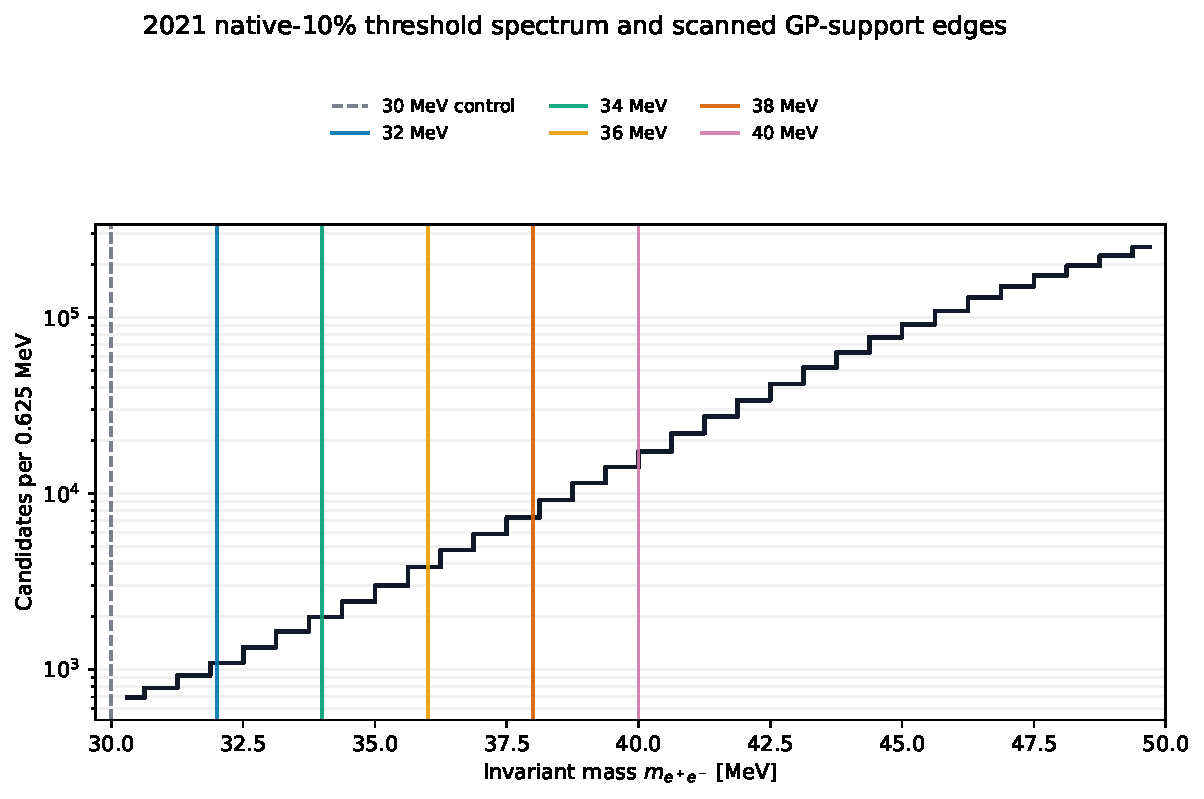
\includegraphics[width=0.98\linewidth]{v4p9p5_support_figs/source_threshold_and_support_edges.pdf}
  \caption{Native 2021 10\% source histogram near threshold.  Vertical lines mark
  the 30~MeV control and the five candidate lower edges of the GP support.  The
  logarithmic vertical scale makes the low-count shoulder and rapid turn-on visible.}
  \label{fig:v4p9p5-source}
\end{figure}

\subsubsection{Initial scan}

The first stage reuses the 100 background-only pseudoexperiments generated from the
fitted source spectrum in the four-exposure study; it does not generate new
pseudo-data. At each support edge, we perform matched-reference extractions at 55,
60, 65, and 70~MeV with 0-, 2-, and 5-$\sigma_A$ injections.
The scan changes only the lower support edge. Binning, preprocessing, blind and
training masks, kernel bounds, signed extraction, and optimizer checks remain fixed as
described in Sections~\ref{sec:methodology} and \ref{sec:toys}. For repeated optimizer
starts, we retain the fit using reproducibility, covariance validity, kernel diagnostics,
and GP log marginal likelihood;
neither the pull nor any limit or $p$-value enters that choice.

The first 25 backgrounds were processed at all six edges. All 1800 fits passed the
numerical checks, with no invalid covariance matrix or contact with a kernel bound.
The original rule rejected an edge if any mass--injection combination had
$|\overline p|\geq0.5$ and a two-sided 90\% Student-$t$ interval that excluded zero.
Every eligible edge failed. Their worst mean-pull magnitudes ranged from 1.072 to
1.530, and the ineligible 30~MeV control reached 1.624. Even the best first-stage
candidate, the 38~MeV edge, was therefore well outside the original 0.5 bound.

\subsubsection{A practical rule and an independent check}

After the first stage, we adopted a less stringent working rule: at least 9 of
the 12 mass--injection means and at least 3 of the 4 zero-signal means had to satisfy
$|\overline p|<0.75$, and no mean could reach 1.25 in magnitude.  The numerical checks,
the minimax score, and the 0.10 tie margin were left unchanged.  Among candidates within
that margin, the lower edge was preferred so that the fit retained more data.  Because
this rule was formulated after the first 25 backgrounds had been examined, it is a
post-selection screen, not a predeclared equivalence test or a test of coverage. It
was fixed before the remaining 75 backgrounds were processed.

Only the 36 and 38~MeV candidates pass the practical rule in the first stage.  The
38~MeV edge has the smaller worst pull, but 36~MeV lies within the retained tie
margin and is therefore selected for confirmation.  The independent continuation uses
backgrounds 25--99 at 34, 36, and 38~MeV. At 36~MeV, 10 of 12 means and all four
zero-signal means satisfy the 0.75 condition in the continuation alone; the worst
magnitude is 0.901.  In the complete 100-background sample, the corresponding counts
are 9 of 12 and 3 of 4, with a worst magnitude of 0.960.  Every fit passes the numerical
checks. With the rule already fixed, we chose 36--300~MeV for the subsequent
2021-only analysis without further tuning.

\begin{figure}[htbp]
  \centering
  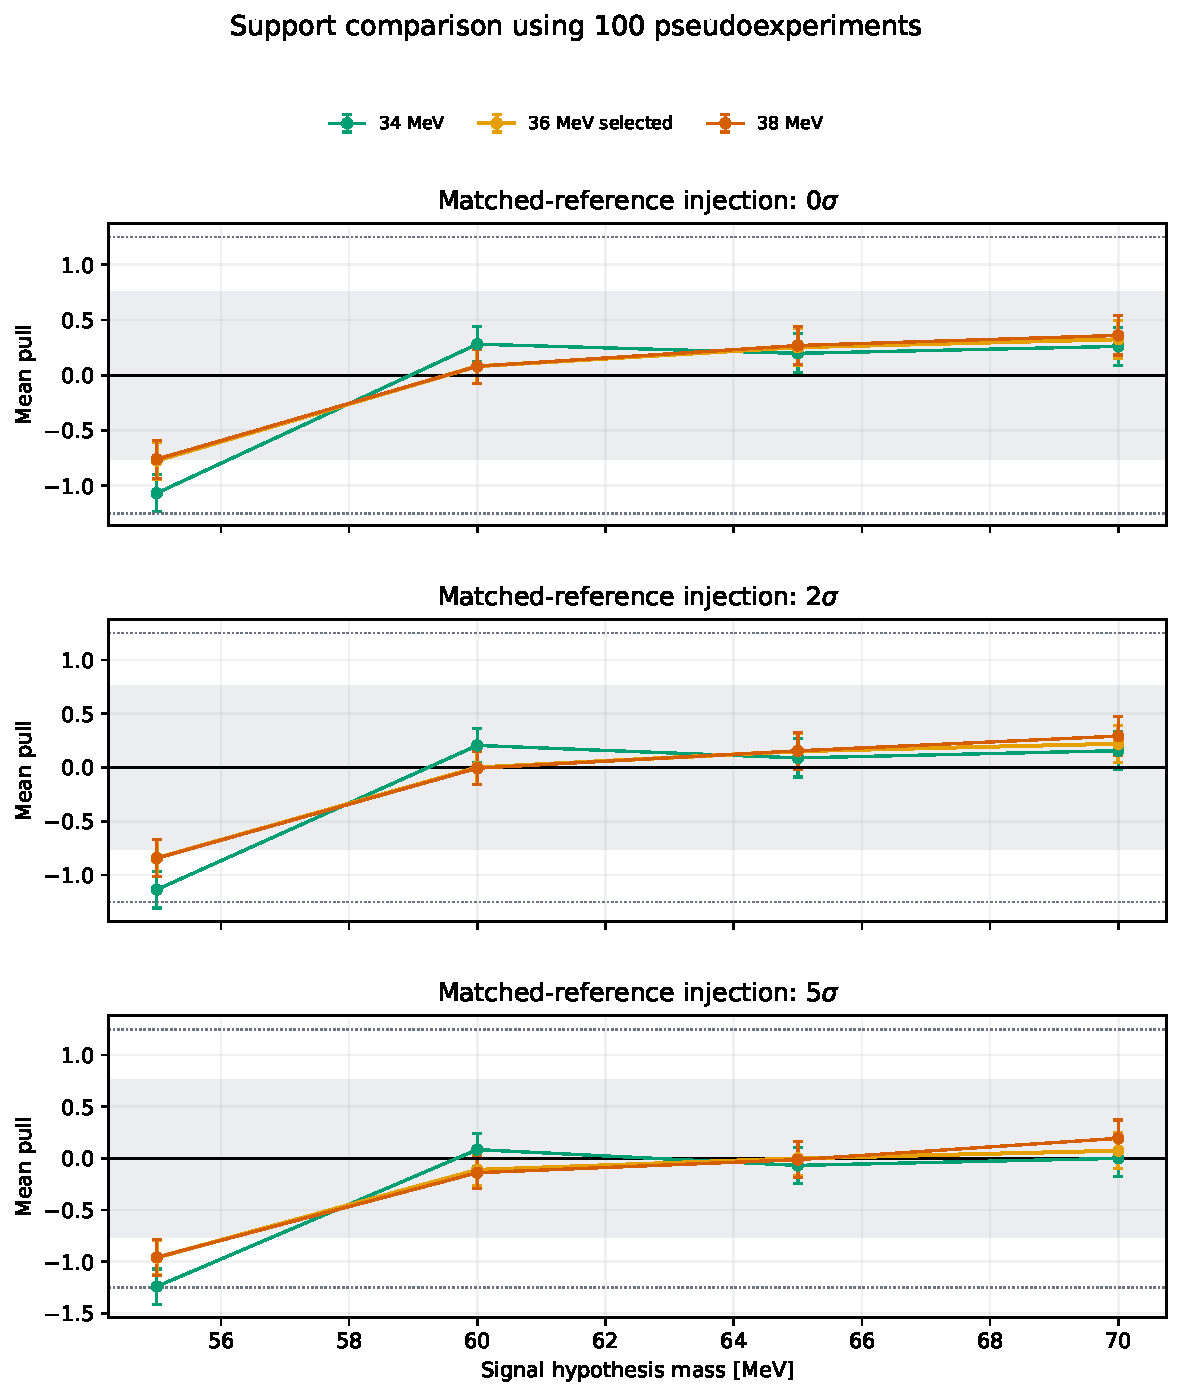
\includegraphics[width=0.98\linewidth]{v4p9p5_support_figs/confirmation_full100_pull_means.pdf}
  \caption{Mean pulls in the complete 100-background sample for the selected edge and
  its two neighboring candidates.  Error bars are two-sided 90\% Student-$t$ intervals
  on the mean.  The shaded band denotes the post-selection $|\overline p|<0.75$
  practical region; dotted lines show the magnitude-1.25 guard.  The remaining
  exceptions are confined to the 55~MeV hypothesis.}
  \label{fig:v4p9p5-confirmation}
\end{figure}

At the selected edge, the full-sample means at 55~MeV are $-0.773$, $-0.841$, and
$-0.960$ for the 0-, 2-, and 5-$\sigma_A$ injections.  Their 90\% intervals exclude
zero, so the low-mass under-recovery is retained as a real limitation of this test.
Across the nine mass--injection combinations from 60 to 70~MeV, the means range from
$-0.110$ to $+0.325$ and
the pull widths from 0.939 to 1.034.  The 65~MeV zero-signal mean is 0.253, with a
90\% interval of $[0.086,0.421]$.

Each numerically valid pseudoexperiment also provides a bounded Wald
$\widetilde q_\mu$ 90\% \CLs{} yield
limit.  We use those values only to check that the limit is stable under nearby support
choices; the smallest limit never determines the selected edge.  This study therefore
supports the 36--300~MeV choice for the declared fitted-source ensemble, with the
55~MeV caveat above.  It does not establish direct coverage or truth-independent
background closure.

\FloatBarrier
